\paragraph{QuizziPedia::Front-End::Views::ResultsView}

\label{QuizziPedia::Front-End::View::ResultView}
\begin{figure} [ht]
	\centering
	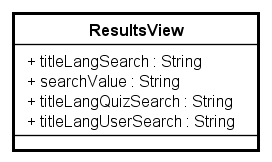
\includegraphics[scale=0.80]{UML/Classi/Front-End/QuizziPedia_Front-end_Views_ResultsView.png}
	\caption{QuizziPedia::Front-End::Views::ResultsView}
\end{figure} \FloatBarrier
\begin{itemize}
	\item \textbf{Descrizione}: \textit{view\ped{G}} contenente i risultati della ricerca effettuata. Vengono visualizzati sia gli utenti che i questionari trovati;
	\item \textbf{Utilizzo}: viene visualizzata dopo aver effettuato un'operazione di ricerca utilizzando \texttt{SearchDirective} e permette di selezionare un risultato presente al suo interno; 
	\item \textbf{Relazioni con altre classi}:
	\begin{itemize}
		\item \textbf{IN \texttt{ResultsModelView}}: classe di tipo \textit{modelview\ped{G}} la cui istanziazione è contenuta all'interno della variabile di ambiente \textit{Angular\ped{G}} All'interno di essa sono presenti le variabili e i metodi necessari per il \textit{Two-Way Data-Binding\ped{G}} tra la \textit{view\ped{G}} \texttt{ResultsView} e il \textit{controller\ped{G}} \texttt{SearchController};
		\item \textbf{IN \texttt{SubscribeResultDirective}}: directive che permette di visualizzare e iscriversi ai questionari ricercati;
		\item \textbf{IN \texttt{UserResultsDirective}}: directive che permette di visualizzare la lista degli utenti ricercati dopo aver utilizzato l'apposita funzione di ricerca;
		\item \textbf{IN \texttt{LangModel}}: rappresenta il modello delle informazioni per la giusta traduzione dell'applicazione.
	\end{itemize}
	\item \textbf{Attributi}:
		\begin{itemize}
			\item \texttt{+ titleLangSearch: String} \\ Attributo che viene utilizzato per visualizzare la giusta traduzione del titolo della pagina, in italiano o in inglese;
			\item \texttt{+ searchValue: String} \\ Attributo che rappresenta la stringa cercata;
			\item \texttt{+ titleLangQuizSearch: String} \\ Attributo che viene utilizzato per visualizzare la giusta traduzione del titolo della sezione questionari, in italiano o in inglese;
			\item \texttt{+ titleLangUserSearch: String} \\ Attributo che viene utilizzato per visualizzare la giusta traduzione del titolo della sezione utenti, in italiano o in inglese.
		\end{itemize}
\end{itemize}